\documentclass[aps,prd,twocolumn,10pt,nofootinbib]{revtex4-2}
% Fallback if revtex is unavailable: \documentclass[twocolumn,10pt]{article} + \usepackage{amsmath,amssymb}
\usepackage{amsmath,amssymb,graphicx}
\usepackage{pgfplots}
\pgfplotsset{compat=1.16}
\usepackage[colorlinks=true,linkcolor=blue,citecolor=blue]{hyperref}

\begin{document}

\title{The External Field Effect:\\ How a Galaxy's Neighbours Reveal Whether Gravity Is Modified}
\author{C.\ Zimmerman}
\date{June 2026}

\begin{abstract}
The \emph{external field effect} (EFE) is the sharpest qualitative test separating modified gravity from
particle dark matter. In Newtonian gravity with a dark halo, a system's internal dynamics are immune to a
\emph{uniform} external field---the shell theorem guarantees it. In Milgromian dynamics (MOND) the field
equation is non-linear, so the internal dynamics \emph{do} depend on the external field: a violation of the
strong equivalence principle that dark matter cannot mimic. We explain the EFE from first principles, derive the
quantitative prediction, and show with worked figures how a strong external field suppresses the
modified-gravity boost and bends the radial acceleration relation back toward Newtonian. The effect is detected
in galaxy rotation curves at $\sim\!4\text{--}5\sigma$. We close by placing it in a geometric framework in which
the acceleration scale is set by the cosmological constant, $a_0=c^2\sqrt{\Lambda/32\pi}$, and the EFE is the
non-locality of the de Sitter horizon's coupling to local matter.
\end{abstract}

\maketitle

\section{Two explanations, one decisive test}
Spiral galaxies rotate too fast for their visible mass: beyond a characteristic acceleration
$a_0\approx1.2\times10^{-10}\,\mathrm{m\,s^{-2}}$ the observed acceleration $g_{\rm obs}$ exceeds the Newtonian
value $g_{\rm bar}$ from baryons alone, following the tight \emph{radial acceleration relation} (RAR), with
$g_{\rm obs}\!\to\!\sqrt{a_0\,g_{\rm bar}}$ at low accelerations~\cite{McGaugh2016}. Two pictures explain this.
\emph{Dark matter}: each galaxy sits in a halo of unseen particles that adds the missing gravity.
\emph{Modified gravity} (MOND~\cite{Milgrom1983}): gravity itself is enhanced below $a_0$, with no new matter.

On rotation curves the two are nearly degenerate. The \emph{external field effect} breaks the degeneracy
cleanly, because it tests a \emph{principle} rather than a fit: does a system's internal gravity care about the
gravitational field of its surroundings?

\section{Why dark matter forbids it, and MOND requires it}
\textbf{Newton $+$ dark matter: no effect.} Newtonian gravity obeys the \emph{strong equivalence principle}: a
spatially uniform external field $\mathbf{g}_{\rm ext}$ accelerates every part of a system equally and cancels
from the internal equations of motion. For a body inside a larger halo, the shell theorem makes the net external
pull vanish in the interior. A dwarf galaxy falling through a cluster has the \emph{same} internal dynamics as
one in deep space. Internal physics is blind to the external field.

\textbf{MOND: an unavoidable effect.} MOND replaces the Poisson equation by a \emph{non-linear} one,
\begin{equation}
\nabla\!\cdot\!\big[\mu(|\nabla\Phi|/a_0)\,\nabla\Phi\big]=4\pi G\rho,
\label{eq:aqual}
\end{equation}
with $\mu(x)\!\to\!1$ for $x\!\gg\!1$ (Newton) and $\mu(x)\!\to\!x$ for $x\!\ll\!1$ (deep-MOND). Non-linearity is
the whole story: in Eq.~\eqref{eq:aqual} one cannot separate the response to internal and external sources. A
constant $\mathbf{g}_{\rm ext}$ shifts the operating point of $\mu$ and therefore changes the \emph{internal}
gravity. The strong equivalence principle is violated---and this is a \emph{prediction}, not a defect.

It is easiest to see in the equivalent quasi-linear formulation (QUMOND). Writing accelerations in units of
$a_0$ and aligning the internal field $g_N$ with the external field $g_{\rm ext}$, the observed internal
acceleration is
\begin{equation}
g_{\rm obs}=\nu(g_N{+}g_{\rm ext})\,(g_N{+}g_{\rm ext})-\nu(g_{\rm ext})\,g_{\rm ext},
\label{eq:efe}
\end{equation}
where $\nu(y)=\tfrac12+\sqrt{\tfrac14+1/y}$ is the interpolation (the inverse of $\mu(x)=x/(1{+}x)$), satisfying
$g_{\rm obs}=\nu\,g$ for an isolated system. For $g_{\rm ext}\!=\!0$ this reduces to the ordinary RAR,
$g_{\rm obs}=\nu(g_N)g_N$, with the deep-MOND limit $g_{\rm obs}=\sqrt{g_N}$ (i.e. $\sqrt{a_0 g_{\rm bar}}$ in
physical units).

\textbf{The key limit.} Deep inside a system ($g_N\!\ll\!g_{\rm ext}$) embedded in a weak external field
($g_{\rm ext}\!<\!1$), expand Eq.~\eqref{eq:efe} to first order in $g_N$:
\begin{equation}
g_{\rm obs}\simeq g_N\,\nu(g_{\rm ext})\Big[1+\tfrac{d\ln\nu}{d\ln g_{\rm ext}}\Big]
\equiv g_N\,\frac{G_{\rm eff}}{G}.
\label{eq:geff}
\end{equation}
The internal dynamics are \emph{Newtonian} but with a renormalised constant $G_{\rm eff}=G\,\nu(g_{\rm ext})
[1+L_e]$ that depends only on the \emph{external} field. As $g_{\rm ext}\!\to\!0$, $\nu\!\to\!\infty$ and the
full MOND boost returns; as $g_{\rm ext}\!\gg\!1$, $\nu\!\to\!1$ and gravity becomes exactly Newtonian. The
external field \emph{erases} the modified-gravity boost.

\section{The prediction, in pictures}
Figure~\ref{fig:rar} plots the RAR from Eq.~\eqref{eq:efe} for an isolated galaxy and for galaxies bathed in
environmental fields of $0.05\,a_0$, $0.2\,a_0$, and $1.0\,a_0$. The isolated curve (blue) climbs above the
Newtonian $1\!:\!1$ line and follows the deep-MOND slope $\tfrac12$, diverging ever further from Newton. A galaxy
in an external field instead \emph{bends to a slope of unity}---parallel to the Newtonian line---once its internal
acceleration falls below $g_{\rm ext}$, settling onto a \emph{plateau} raised above Newton by the factor
$\nu(g_{\rm ext})$. The stronger the environment, the lower the plateau; for $g_{\rm ext}\!\gtrsim\!a_0$ it sits
essentially on the Newtonian line. This environment-dependent flattening is the EFE's signature, and it is
impossible in the dark-matter picture.

\begin{figure}[t]
\centering
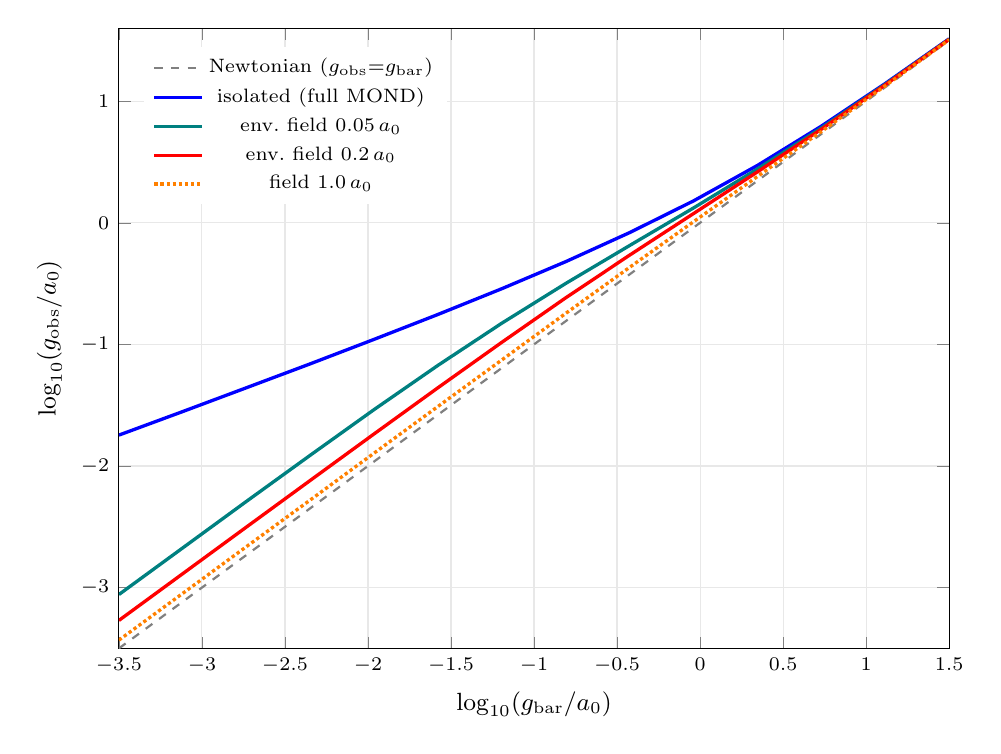
\begin{tikzpicture}
\begin{axis}[width=\columnwidth,height=0.78\columnwidth,
  xlabel={$\log_{10}(g_{\rm bar}/a_0)$}, ylabel={$\log_{10}(g_{\rm obs}/a_0)$},
  legend pos=north west, legend style={font=\scriptsize,draw=none},
  grid=both, grid style={gray!18}, xmin=-3.5, xmax=1.5, ymin=-3.5, ymax=1.6,
  tick label style={font=\scriptsize}, label style={font=\small}]
\addplot[dashed,gray,thick,domain=-3.5:1.5,samples=2]{x}; \addlegendentry{Newtonian ($g_{\rm obs}{=}g_{\rm bar}$)}
\addplot[blue,very thick] coordinates {(-3.500,-1.746)(-3.115,-1.552)(-2.731,-1.356)(-2.346,-1.159)(-1.962,-0.958)(-1.577,-0.753)(-1.192,-0.541)(-0.808,-0.319)(-0.423,-0.080)(-0.038,0.181)(0.346,0.472)(0.731,0.795)(1.115,1.145)(1.500,1.513)};
\addlegendentry{isolated (full MOND)}
\addplot[teal,very thick] coordinates {(-3.500,-3.057)(-3.115,-2.673)(-2.731,-2.290)(-2.346,-1.910)(-1.962,-1.535)(-1.577,-1.171)(-1.192,-0.824)(-0.808,-0.498)(-0.423,-0.186)(-0.038,0.123)(0.346,0.443)(0.731,0.781)(1.115,1.139)(1.500,1.510)};
\addlegendentry{env.\ field $0.05\,a_0$}
\addplot[red,very thick] coordinates {(-3.500,-3.270)(-3.115,-2.885)(-2.731,-2.501)(-2.346,-2.117)(-1.962,-1.735)(-1.577,-1.355)(-1.192,-0.981)(-0.808,-0.616)(-0.423,-0.265)(-0.038,0.077)(0.346,0.419)(0.731,0.770)(1.115,1.134)(1.500,1.508)};
\addlegendentry{env.\ field $0.2\,a_0$}
\addplot[orange,very thick,densely dotted] coordinates {(-3.500,-3.432)(-3.115,-3.047)(-2.731,-2.662)(-2.346,-2.278)(-1.962,-1.893)(-1.577,-1.509)(-1.192,-1.126)(-0.808,-0.744)(-0.423,-0.365)(-0.038,0.010)(0.346,0.381)(0.731,0.751)(1.115,1.126)(1.500,1.505)};
\addlegendentry{field $1.0\,a_0$}
\end{axis}
\end{tikzpicture}
\caption{The radial acceleration relation with the external field effect. An isolated galaxy (blue) keeps lifting
away from the Newtonian line (deep-MOND slope $\tfrac12$); a galaxy in an environmental field bends to a
\emph{plateau} parallel to Newton, raised by $\nu(g_{\rm ext})$ and lowered as the field strengthens. The
dependence on the \emph{environment} is forbidden for Newton$+$dark matter.}
\label{fig:rar}
\end{figure}

Figure~\ref{fig:boost} isolates the magnitude: the internal ``boost'' $g_{\rm obs}/g_{\rm bar}$ measured deep in
the MOND regime ($g_{\rm bar}=0.01\,a_0$) as a function of the external field. With no external field the boost
is $\sim\!10$ (the deep-MOND $\sqrt{a_0/g_{\rm bar}}$); a Milky-Way-like field ($1.8\,a_0$) already cuts it to
$1.09$; a strong field drives it to unity (Newtonian). \emph{A system's internal gravity is dialled by its
neighbours.}

\begin{figure}[t]
\centering
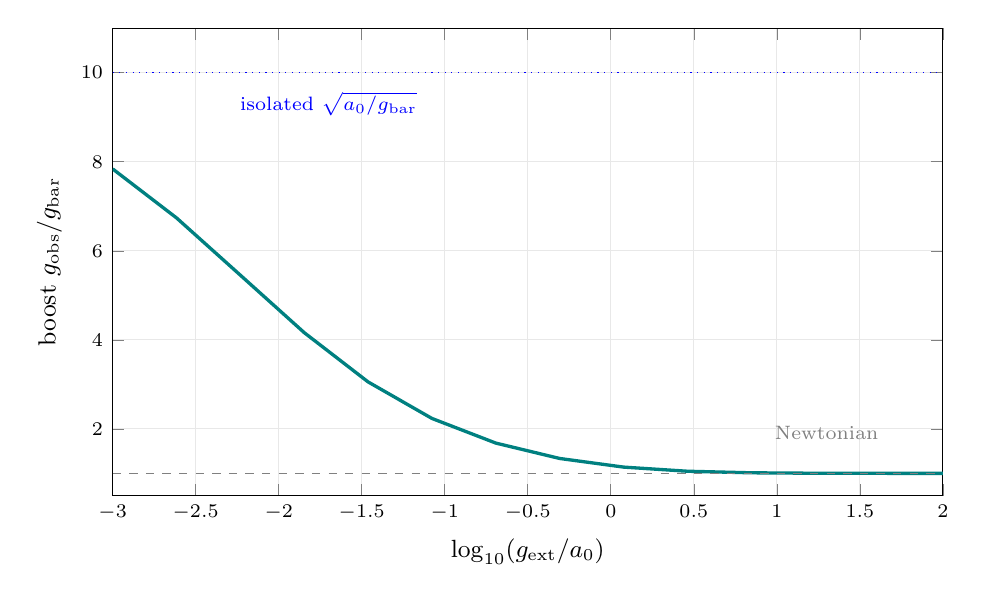
\begin{tikzpicture}
\begin{axis}[width=\columnwidth,height=0.62\columnwidth,
  xlabel={$\log_{10}(g_{\rm ext}/a_0)$}, ylabel={boost $g_{\rm obs}/g_{\rm bar}$},
  grid=both, grid style={gray!18}, xmin=-3, xmax=2, ymin=0.5, ymax=11,
  tick label style={font=\scriptsize}, label style={font=\small}]
\addplot[teal,very thick] coordinates {(-3.000,7.840)(-2.615,6.738)(-2.231,5.453)(-1.846,4.161)(-1.462,3.056)(-1.077,2.234)(-0.692,1.680)(-0.308,1.335)(0.077,1.141)(0.462,1.048)(0.846,1.013)(1.231,1.003)(1.615,1.001)(2.000,1.000)};
\addplot[dotted,blue,domain=-3:2,samples=2]{10}; \node[font=\scriptsize,blue] at (axis cs:-1.7,9.3){isolated $\sqrt{a_0/g_{\rm bar}}$};
\addplot[dashed,gray,domain=-3:2,samples=2]{1}; \node[font=\scriptsize,gray] at (axis cs:1.3,1.9){Newtonian};
\end{axis}
\end{tikzpicture}
\caption{The modified-gravity boost deep in the MOND regime ($g_{\rm bar}=0.01\,a_0$) collapses from $\sim\!10$
(isolated) to $1$ (Newtonian) as the external field strengthens past $a_0$.}
\label{fig:boost}
\end{figure}

\section{It is observed}
The prediction is concrete: galaxies in stronger external fields should show a more pronounced low-acceleration
downturn in their RAR. Analysing the SPARC database of rotation curves with environmental field estimates, Chae
and collaborators report exactly this signature at $\sim\!4\text{--}5\sigma$~\cite{Chae2021}. The complementary
laboratory is the Milky Way's \emph{wide binary stars} (separations $\gtrsim\!7000\,$AU), whose internal
accelerations fall below $a_0$ while sitting in the Galaxy's external field of $\approx\!1.8\,a_0$: the framework
here predicts a small residual boost ($\sim\!+5\%$), between zero (dark matter) and the isolated MOND value;
Gaia astrometry is now testing it~\cite{Banik2024}. No detection is yet decisive, but the \emph{qualitative}
EFE---internal dynamics that depend on the environment---is a clean discriminator that has, so far, gone the way
modified gravity predicts.

\section{Where $a_0$ comes from}
The EFE inherits its scale $a_0$ from cosmology. In a universe with a cosmological constant $\Lambda>0$, the de
Sitter horizon has curvature $\sqrt{\Lambda}$, and the emergent-gravity acceleration it sets is
\begin{equation}
a_0=c^2\sqrt{\Lambda/32\pi}=cH(z)/Z,\qquad Z=2\sqrt{8\pi/3},
\label{eq:a0}
\end{equation}
the long-noted coincidence $a_0\!\approx\!cH_0$ made precise (Eq.~\eqref{eq:a0} gives
$a_0\!=\!0.9\text{--}1.1\times10^{-10}\,\mathrm{m\,s^{-2}}$ for the observed $\Lambda$). In this reading the EFE
is the \emph{non-locality of the horizon's coupling}: because the modified dynamics descend from the global de
Sitter geometry rather than from local mass alone, the field an object sits in---set partly by its
neighbours---enters its internal physics. Dark energy ($\Lambda$) and ``dark matter'' (the MOND boost) are then
two faces of one geometry.

\section{Conclusion}
The external field effect is the cleanest fork in the dark-sector road. Newtonian gravity plus dark matter
\emph{cannot} make a system's internal dynamics depend on a uniform external field; MOND \emph{must}. We derived
the effect from the non-linear field equation, showed how a strong external field erases the modified-gravity
boost and bends the RAR back to Newtonian (Figs.~\ref{fig:rar}--\ref{fig:boost}), and noted its
$\sim\!4\text{--}5\sigma$ detection. Whatever ultimately explains galactic dynamics must reckon with a fact dark
matter does not predict: \emph{a galaxy's gravity knows about its neighbours.}

\begin{thebibliography}{9}
\bibitem{McGaugh2016} S.~McGaugh, F.~Lelli, J.~Schombert, Phys.\ Rev.\ Lett.\ \textbf{117}, 201101 (2016).
\bibitem{Milgrom1983} M.~Milgrom, Astrophys.\ J.\ \textbf{270}, 365 (1983).
\bibitem{Chae2021} K.-H.~Chae \emph{et al.}, Astrophys.\ J.\ \textbf{904}, 51 (2020); \textbf{921}, 104 (2021).
\bibitem{Banik2024} I.~Banik \emph{et al.}, MNRAS \textbf{527}, 4573 (2024); K.-H.~Chae, ApJ \textbf{960}, 114 (2024).
\end{thebibliography}

\end{document}
